% Options for packages loaded elsewhere
\PassOptionsToPackage{unicode}{hyperref}
\PassOptionsToPackage{hyphens}{url}
%
\documentclass[
]{book}
\usepackage{lmodern}
\usepackage{amsmath}
\usepackage{ifxetex,ifluatex}
\ifnum 0\ifxetex 1\fi\ifluatex 1\fi=0 % if pdftex
  \usepackage[T1]{fontenc}
  \usepackage[utf8]{inputenc}
  \usepackage{textcomp} % provide euro and other symbols
  \usepackage{amssymb}
\else % if luatex or xetex
  \usepackage{unicode-math}
  \defaultfontfeatures{Scale=MatchLowercase}
  \defaultfontfeatures[\rmfamily]{Ligatures=TeX,Scale=1}
\fi
% Use upquote if available, for straight quotes in verbatim environments
\IfFileExists{upquote.sty}{\usepackage{upquote}}{}
\IfFileExists{microtype.sty}{% use microtype if available
  \usepackage[]{microtype}
  \UseMicrotypeSet[protrusion]{basicmath} % disable protrusion for tt fonts
}{}
\makeatletter
\@ifundefined{KOMAClassName}{% if non-KOMA class
  \IfFileExists{parskip.sty}{%
    \usepackage{parskip}
  }{% else
    \setlength{\parindent}{0pt}
    \setlength{\parskip}{6pt plus 2pt minus 1pt}}
}{% if KOMA class
  \KOMAoptions{parskip=half}}
\makeatother
\usepackage{xcolor}
\IfFileExists{xurl.sty}{\usepackage{xurl}}{} % add URL line breaks if available
\IfFileExists{bookmark.sty}{\usepackage{bookmark}}{\usepackage{hyperref}}
\hypersetup{
  pdftitle={5장 랜덤화 블럭설계, 라틴정방설계와 분할법 - 예제},
  pdfauthor={서울시립대 통계학과},
  hidelinks,
  pdfcreator={LaTeX via pandoc}}
\urlstyle{same} % disable monospaced font for URLs
\usepackage{color}
\usepackage{fancyvrb}
\newcommand{\VerbBar}{|}
\newcommand{\VERB}{\Verb[commandchars=\\\{\}]}
\DefineVerbatimEnvironment{Highlighting}{Verbatim}{commandchars=\\\{\}}
% Add ',fontsize=\small' for more characters per line
\usepackage{framed}
\definecolor{shadecolor}{RGB}{248,248,248}
\newenvironment{Shaded}{\begin{snugshade}}{\end{snugshade}}
\newcommand{\AlertTok}[1]{\textcolor[rgb]{0.94,0.16,0.16}{#1}}
\newcommand{\AnnotationTok}[1]{\textcolor[rgb]{0.56,0.35,0.01}{\textbf{\textit{#1}}}}
\newcommand{\AttributeTok}[1]{\textcolor[rgb]{0.77,0.63,0.00}{#1}}
\newcommand{\BaseNTok}[1]{\textcolor[rgb]{0.00,0.00,0.81}{#1}}
\newcommand{\BuiltInTok}[1]{#1}
\newcommand{\CharTok}[1]{\textcolor[rgb]{0.31,0.60,0.02}{#1}}
\newcommand{\CommentTok}[1]{\textcolor[rgb]{0.56,0.35,0.01}{\textit{#1}}}
\newcommand{\CommentVarTok}[1]{\textcolor[rgb]{0.56,0.35,0.01}{\textbf{\textit{#1}}}}
\newcommand{\ConstantTok}[1]{\textcolor[rgb]{0.00,0.00,0.00}{#1}}
\newcommand{\ControlFlowTok}[1]{\textcolor[rgb]{0.13,0.29,0.53}{\textbf{#1}}}
\newcommand{\DataTypeTok}[1]{\textcolor[rgb]{0.13,0.29,0.53}{#1}}
\newcommand{\DecValTok}[1]{\textcolor[rgb]{0.00,0.00,0.81}{#1}}
\newcommand{\DocumentationTok}[1]{\textcolor[rgb]{0.56,0.35,0.01}{\textbf{\textit{#1}}}}
\newcommand{\ErrorTok}[1]{\textcolor[rgb]{0.64,0.00,0.00}{\textbf{#1}}}
\newcommand{\ExtensionTok}[1]{#1}
\newcommand{\FloatTok}[1]{\textcolor[rgb]{0.00,0.00,0.81}{#1}}
\newcommand{\FunctionTok}[1]{\textcolor[rgb]{0.00,0.00,0.00}{#1}}
\newcommand{\ImportTok}[1]{#1}
\newcommand{\InformationTok}[1]{\textcolor[rgb]{0.56,0.35,0.01}{\textbf{\textit{#1}}}}
\newcommand{\KeywordTok}[1]{\textcolor[rgb]{0.13,0.29,0.53}{\textbf{#1}}}
\newcommand{\NormalTok}[1]{#1}
\newcommand{\OperatorTok}[1]{\textcolor[rgb]{0.81,0.36,0.00}{\textbf{#1}}}
\newcommand{\OtherTok}[1]{\textcolor[rgb]{0.56,0.35,0.01}{#1}}
\newcommand{\PreprocessorTok}[1]{\textcolor[rgb]{0.56,0.35,0.01}{\textit{#1}}}
\newcommand{\RegionMarkerTok}[1]{#1}
\newcommand{\SpecialCharTok}[1]{\textcolor[rgb]{0.00,0.00,0.00}{#1}}
\newcommand{\SpecialStringTok}[1]{\textcolor[rgb]{0.31,0.60,0.02}{#1}}
\newcommand{\StringTok}[1]{\textcolor[rgb]{0.31,0.60,0.02}{#1}}
\newcommand{\VariableTok}[1]{\textcolor[rgb]{0.00,0.00,0.00}{#1}}
\newcommand{\VerbatimStringTok}[1]{\textcolor[rgb]{0.31,0.60,0.02}{#1}}
\newcommand{\WarningTok}[1]{\textcolor[rgb]{0.56,0.35,0.01}{\textbf{\textit{#1}}}}
\usepackage{longtable,booktabs}
\usepackage{calc} % for calculating minipage widths
% Correct order of tables after \paragraph or \subparagraph
\usepackage{etoolbox}
\makeatletter
\patchcmd\longtable{\par}{\if@noskipsec\mbox{}\fi\par}{}{}
\makeatother
% Allow footnotes in longtable head/foot
\IfFileExists{footnotehyper.sty}{\usepackage{footnotehyper}}{\usepackage{footnote}}
\makesavenoteenv{longtable}
\usepackage{graphicx}
\makeatletter
\def\maxwidth{\ifdim\Gin@nat@width>\linewidth\linewidth\else\Gin@nat@width\fi}
\def\maxheight{\ifdim\Gin@nat@height>\textheight\textheight\else\Gin@nat@height\fi}
\makeatother
% Scale images if necessary, so that they will not overflow the page
% margins by default, and it is still possible to overwrite the defaults
% using explicit options in \includegraphics[width, height, ...]{}
\setkeys{Gin}{width=\maxwidth,height=\maxheight,keepaspectratio}
% Set default figure placement to htbp
\makeatletter
\def\fps@figure{htbp}
\makeatother
\setlength{\emergencystretch}{3em} % prevent overfull lines
\providecommand{\tightlist}{%
  \setlength{\itemsep}{0pt}\setlength{\parskip}{0pt}}
\setcounter{secnumdepth}{5}
\usepackage[onehalfspacing]{setspace}

\usepackage[hangul]{kotex}
\usepackage{fullpage}
\newcommand{\pardiff}[2]{\frac{\partial #1}{\partial #2 }}
\newcommand{\pardiffl}[2]{{\partial #1}/{\partial #2 }}
\newcommand{\pardiffd}[2]{\frac{\partial^2 #1}{\partial #2^t \partial #2 }}
\newcommand{\pardiffdd}[3]{\frac{\partial^2 #1}{\partial #2 \partial #3 }}

\newcommand{\bm}[1]{ \symbf{#1}}

\usepackage{booktabs}
\usepackage{longtable}
\usepackage[bf,singlelinecheck=off]{caption}

%\setmainfont[UprightFeatures={SmallCapsFont=AlegreyaSC-Regular}]{Alegreya}

\usepackage{framed,color}
\definecolor{shadecolor}{RGB}{248,248,248}

\renewcommand{\textfraction}{0.05}
\renewcommand{\topfraction}{0.8}
\renewcommand{\bottomfraction}{0.8}
\renewcommand{\floatpagefraction}{0.75}

\renewenvironment{quote}{\begin{VF}}{\end{VF}}
\let\oldhref\href
\renewcommand{\href}[2]{#2\footnote{\url{#1}}}

\makeatletter
\newenvironment{kframe}{%
\medskip{}
\setlength{\fboxsep}{.8em}
 \def\at@end@of@kframe{}%
 \ifinner\ifhmode%
  \def\at@end@of@kframe{\end{minipage}}%
  \begin{minipage}{\columnwidth}%
 \fi\fi%
 \def\FrameCommand##1{\hskip\@totalleftmargin \hskip-\fboxsep
 \colorbox{shadecolor}{##1}\hskip-\fboxsep
     % There is no \\@totalrightmargin, so:
     \hskip-\linewidth \hskip-\@totalleftmargin \hskip\columnwidth}%
 \MakeFramed {\advance\hsize-\width
   \@totalleftmargin\z@ \linewidth\hsize
   \@setminipage}}%
 {\par\unskip\endMakeFramed%
 \at@end@of@kframe}
\makeatother

\makeatletter

\@ifundefined{Shaded}{
}{\renewenvironment{Shaded}{\begin{kframe}}{\end{kframe}}}
\makeatother

\newenvironment{rmdblock}[1]
  {
  \begin{itemize}
  \renewcommand{\labelitemi}{
    \raisebox{-.7\height}[0pt][0pt]{
      {\setkeys{Gin}{width=3em,keepaspectratio}\includegraphics{images/#1}}
    }
  }
  \setlength{\fboxsep}{1em}
  \begin{kframe}
  \item
  }
  {
  \end{kframe}
  \end{itemize}
  }
  
\newenvironment{rmdnote}
  {\begin{rmdblock}{note}}
  {\end{rmdblock}}
  
\newenvironment{rmdcaution}
  {\begin{rmdblock}{caution}}
  {\end{rmdblock}}
  
\newenvironment{rmdimportant}
  {\begin{rmdblock}{important}}
  {\end{rmdblock}}
  
\newenvironment{rmdtip}
  {\begin{rmdblock}{tip}}
  {\end{rmdblock}}
  
\newenvironment{rmdwarning}
  {\begin{rmdblock}{warning}}
  {\end{rmdblock}}
  


%\usepackage{makeidx}
%\makeindex

\urlstyle{tt}

\usepackage{amsthm}
\makeatletter
 \def\thm@space@setup{%
   \thm@preskip=8pt plus 2pt minus 4pt
   \thm@postskip=\thm@preskip
}
\makeatother

\frontmatter

\ifluatex
  \usepackage{selnolig}  % disable illegal ligatures
\fi
\usepackage[]{natbib}
\bibliographystyle{apalike}

\title{5장 랜덤화 블럭설계, 라틴정방설계와 분할법 - 예제}
\author{서울시립대 통계학과}
\date{2021-04-01}

\begin{document}
\maketitle

{
\setcounter{tocdepth}{1}
\tableofcontents
}
\hypertarget{uxc11cuxbb38}{%
\chapter*{서문}\label{uxc11cuxbb38}}


5장에 이원배치법에 대한 예제, R 프로그램과 결과 해석에 대한 강의자료입니다.

이 노트에 있는 R 프로그램을 실행하려면 다음과 같은 패키지들이 필요하다.

\begin{verbatim}
library(dplyr)
library(tidyr)
library(ggplot2)
library(ggbeeswarm)
library(agricolae)
library(lme4)
library(lmerTest)
\end{verbatim}

\mainmatter

\hypertarget{ex51}{%
\chapter{랜덤화 블럭설계}\label{ex51}}

\hypertarget{uxc2e4uxd5d8uxacc4uxd68d-uxc608uxc81c-5.1--uxd50cuxb77cuxc2a4uxd2f1-uxac15uxb3c4}{%
\section{실험계획: 예제 5.1 -플라스틱 강도}\label{uxc2e4uxd5d8uxacc4uxd68d-uxc608uxc81c-5.1--uxd50cuxb77cuxc2a4uxd2f1-uxac15uxb3c4}}

플라스틱 제품의 강도를 측정하는 것이 실험의 목적이다. 랜덤하게 4일을 택해서 각 일마다 온도를 3개 수준으로 랜덤하게 변화시켜서 제품의 강도(\texttt{intensity})를 측정하였다.

여기서 온도(\texttt{temp})는 고정효과(\(\tau\))이며 선택된 일(\texttt{day})는 블럭(\(\rho\))에 따른 효과이다.

\[ x_{ij} = \mu + \tau_i + \rho_j + e_{ij} \]

\hypertarget{uxc790uxb8ccuxc758-uxad6cuxc131}{%
\section{자료의 구성}\label{uxc790uxb8ccuxc758-uxad6cuxc131}}

이제 실험자료를 입력하여 데이터프레임으로 만들어 보자

\begin{Shaded}
\begin{Highlighting}[]
\NormalTok{intensity}\OtherTok{\textless{}{-}} \FunctionTok{c}\NormalTok{(}\FloatTok{98.0}\NormalTok{, }\FloatTok{97.7}\NormalTok{, }\FloatTok{96.5}\NormalTok{,}
              \FloatTok{99.0}\NormalTok{, }\FloatTok{98.0}\NormalTok{, }\FloatTok{97.9}\NormalTok{,}
              \FloatTok{98.6}\NormalTok{, }\FloatTok{98.2}\NormalTok{, }\FloatTok{96.9}\NormalTok{,}
              \FloatTok{97.6}\NormalTok{, }\FloatTok{97.3}\NormalTok{, }\FloatTok{96.7}\NormalTok{)}

\NormalTok{temp}\OtherTok{\textless{}{-}} \FunctionTok{factor}\NormalTok{(}\FunctionTok{rep}\NormalTok{(}\FunctionTok{c}\NormalTok{(}\DecValTok{70}\NormalTok{, }\DecValTok{80}\NormalTok{, }\DecValTok{90}\NormalTok{), }\AttributeTok{times=}\DecValTok{4}\NormalTok{))}
\NormalTok{day}\OtherTok{\textless{}{-}} \FunctionTok{as.factor}\NormalTok{(}\FunctionTok{rep}\NormalTok{(}\FunctionTok{c}\NormalTok{(}\DecValTok{1}\SpecialCharTok{:}\DecValTok{4}\NormalTok{), }\AttributeTok{each=}\DecValTok{3}\NormalTok{))}

\NormalTok{df}\OtherTok{\textless{}{-}} \FunctionTok{data.frame}\NormalTok{(}\AttributeTok{intensity=}\NormalTok{intensity, }\AttributeTok{temp=}\NormalTok{temp, }\AttributeTok{day=}\NormalTok{day)}
\NormalTok{df}
\end{Highlighting}
\end{Shaded}

\begin{verbatim}
##    intensity temp day
## 1       98.0   70   1
## 2       97.7   80   1
## 3       96.5   90   1
## 4       99.0   70   2
## 5       98.0   80   2
## 6       97.9   90   2
## 7       98.6   70   3
## 8       98.2   80   3
## 9       96.9   90   3
## 10      97.6   70   4
## 11      97.3   80   4
## 12      96.7   90   4
\end{verbatim}

벡터를 범주형 변수로 만들어 줄때 두 함수 \texttt{as.factor()} 와 \texttt{factor()} 모두 사용 가능하다.

\hypertarget{uxc2dcuxac01uxc801-uxbd84uxc11d}{%
\section{시각적 분석}\label{uxc2dcuxac01uxc801-uxbd84uxc11d}}

이제 온도의 수준에 따른 변화를 볼 수 있는 그림을 그려보자. 온도가 올라가면 강도가 떨어지는 경향을 볼 수 있다.

\begin{Shaded}
\begin{Highlighting}[]
\NormalTok{df }\SpecialCharTok{\%\textgreater{}\%} 
  \FunctionTok{ggplot}\NormalTok{(}\FunctionTok{aes}\NormalTok{(}\AttributeTok{x =}\NormalTok{ temp  , }\AttributeTok{y =}\NormalTok{ intensity,  }\AttributeTok{color=}\NormalTok{day)) }\SpecialCharTok{+}
   \FunctionTok{geom\_line}\NormalTok{(}\FunctionTok{aes}\NormalTok{(}\AttributeTok{group =}\NormalTok{ day)) }\SpecialCharTok{+}   \FunctionTok{geom\_point}\NormalTok{()}
\end{Highlighting}
\end{Shaded}

\includegraphics{chapter05_files/figure-latex/unnamed-chunk-3-1.pdf}

\begin{Shaded}
\begin{Highlighting}[]
\FunctionTok{plot}\NormalTok{(intensity }\SpecialCharTok{\textasciitilde{}}\NormalTok{ temp, }\AttributeTok{data=}\NormalTok{df)}
\end{Highlighting}
\end{Shaded}

\includegraphics{chapter05_files/figure-latex/unnamed-chunk-4-1.pdf}

이제 실험일에 따른 변동을 살펴보자. 실험일에 따라서 온도의 효과가 변하는 것을 볼 수 있다.
단 실험일과 온도의 상호작용은 크게 나타나지 않는다. 유의할 점은 반복이 없기 때문에 상호작용에 대한 추론은 불가능하다

\begin{Shaded}
\begin{Highlighting}[]
\NormalTok{df }\SpecialCharTok{\%\textgreater{}\%} 
  \FunctionTok{ggplot}\NormalTok{(}\FunctionTok{aes}\NormalTok{(}\AttributeTok{x =}\NormalTok{ day  , }\AttributeTok{y =}\NormalTok{ intensity,  }\AttributeTok{color=}\NormalTok{temp)) }\SpecialCharTok{+}
   \FunctionTok{geom\_line}\NormalTok{(}\FunctionTok{aes}\NormalTok{(}\AttributeTok{group =}\NormalTok{ temp)) }\SpecialCharTok{+}   \FunctionTok{geom\_point}\NormalTok{()}
\end{Highlighting}
\end{Shaded}

\includegraphics{chapter05_files/figure-latex/unnamed-chunk-5-1.pdf}

\hypertarget{uxbd84uxc0b0uxbd84uxc11d}{%
\section{분산분석}\label{uxbd84uxc0b0uxbd84uxc11d}}

\textbf{블럭 효과인 실험일(\texttt{day})를 고정효과}로 놓았을 경우 분산분석표는 다음과 같다.

\[ \rho_j : \text{ fixed effect,}  \quad e_{ij} \sim N(0, \sigma_E^2) \]

\begin{Shaded}
\begin{Highlighting}[]
\NormalTok{model}\OtherTok{\textless{}{-}} \FunctionTok{aov}\NormalTok{(intensity }\SpecialCharTok{\textasciitilde{}}\NormalTok{ temp }\SpecialCharTok{+}\NormalTok{ day, }\AttributeTok{data=}\NormalTok{df)}
\FunctionTok{summary}\NormalTok{(model)}
\end{Highlighting}
\end{Shaded}

\begin{verbatim}
##             Df Sum Sq Mean Sq F value Pr(>F)   
## temp         2   3.44   1.720   18.43 0.0027 **
## day          3   2.22   0.740    7.93 0.0165 * 
## Residuals    6   0.56   0.093                  
## ---
## Signif. codes:  0 '***' 0.001 '**' 0.01 '*' 0.05 '.' 0.1 ' ' 1
\end{verbatim}

위의 분산분석표에서 온도의 효과를 검정하는 F-통계량의 값은 18.4286 이고 p-값은 0.0027이다. 따라서 5\% 유의수준으로 귀무가설을 기각하며 온도에 따라서 강도는 유의하게 다르다.

일반적으로 블럭효과에 대해서는 검정하지 않지만 그래도 p-값이 0.0165 로서 매우 작으므로 실험일에 따른 변동이 크다는 것을 알 수 있다. 이는 실험울 수행하는 날에 따라서 관측값에 변동이 크다는 것이다. 단 상호작용이 그림으로 볼 때 나타나지 않기 때문에 온도의 효과는 적절하게 추정할 수 있다.

\hypertarget{uxd63cuxd569uxbaa8uxd615}{%
\section{혼합모형}\label{uxd63cuxd569uxbaa8uxd615}}

고정효과와 임의효과(변량)가 동시에 모형식에 나타나는 모형을 혼합모형(mixed models)이라고 부른다.

\begin{itemize}
\item
  혼합모형을 적합시키는 패키지는 \texttt{lme4} 이며 모형을 적합시키는 함수는 \texttt{lmer}이다.
\item
  혼합모형으로 부터 얻은 분산분석표에서 p-값을 보려면 패키지 \texttt{lmerTest}를 사용해야 한다.
\item
  함수 \texttt{lmer} 에서 고정효과에 대한 모형식은 함수 \texttt{anova}와 같다.
\item
  함수 \texttt{lmer} 에서 만약 변수 \texttt{var} 을 임의효과로 고려하려면 \texttt{(1\textbar{}var)} 으로 쓰면 된다.
\end{itemize}

다음은 플라스틱 강도 자료 실험에서 \textbf{블럭 효과인 실험일(\texttt{day}, \(\rho\))를 임의효과}로 놓았을 경우 분석결과이다. 즉

\[ \rho_j \sim N(0, \sigma_B^2), \quad e_{ij} \sim N(0, \sigma_E^2) \]

\begin{Shaded}
\begin{Highlighting}[]
\NormalTok{fit }\OtherTok{\textless{}{-}} \FunctionTok{lmer}\NormalTok{(intensity }\SpecialCharTok{\textasciitilde{}}\NormalTok{ temp }\SpecialCharTok{+}\NormalTok{ (}\DecValTok{1}\SpecialCharTok{|}\NormalTok{day), }\AttributeTok{data=}\NormalTok{df)}
\FunctionTok{summary}\NormalTok{(fit)}
\end{Highlighting}
\end{Shaded}

\begin{verbatim}
## Linear mixed model fit by REML. t-tests use Satterthwaite's method [
## lmerModLmerTest]
## Formula: intensity ~ temp + (1 | day)
##    Data: df
## 
## REML criterion at convergence: 14.6
## 
## Scaled residuals: 
##    Min     1Q Median     3Q    Max 
## -1.062 -0.799  0.143  0.542  1.230 
## 
## Random effects:
##  Groups   Name        Variance Std.Dev.
##  day      (Intercept) 0.2156   0.464   
##  Residual             0.0933   0.306   
## Number of obs: 12, groups:  day, 4
## 
## Fixed effects:
##             Estimate Std. Error     df t value Pr(>|t|)    
## (Intercept)   98.300      0.278  4.559  353.74  2.7e-11 ***
## temp80        -0.500      0.216  6.000   -2.31  0.05989 .  
## temp90        -1.300      0.216  6.000   -6.02  0.00095 ***
## ---
## Signif. codes:  0 '***' 0.001 '**' 0.01 '*' 0.05 '.' 0.1 ' ' 1
## 
## Correlation of Fixed Effects:
##        (Intr) temp80
## temp80 -0.389       
## temp90 -0.389  0.500
\end{verbatim}

위의 결과에서 블럭효과(\texttt{day}) 를 나타내는 분산 성분 \(\sigma_B^2\)의 추정치는 0.2156 이며 오차항(\texttt{Residual})의 분산 \(\sigma_E^2\)의 추정치는 0.0933 이다. 이는 급내상관 계수(ICC)는 0.6978 로서 매우 크다는 것을 의미한다.

\[ ICC = \frac{\sigma_B^2}{\sigma_B^2 + \sigma_E^2} =  0.6978 \]

다음은 플라스틱 강도 자료 실험에서 블럭 효과를 임의효과로 놓았을 경우 분산분석표이다.
함수 \texttt{lmer} 에 의해 생성된 결과를 함수 \texttt{anova}에 적용하면 고정효과에 대한 분산분석과 F-검정만 보여준다. 앞에서 블럭을 고정효과로 놓았을 때 분산분석의 검정 결과와 같다.

\begin{Shaded}
\begin{Highlighting}[]
\FunctionTok{anova}\NormalTok{(fit)}
\end{Highlighting}
\end{Shaded}

\begin{verbatim}
## Type III Analysis of Variance Table with Satterthwaite's method
##      Sum Sq Mean Sq NumDF DenDF F value Pr(>F)   
## temp   3.44    1.72     2     6    18.4 0.0027 **
## ---
## Signif. codes:  0 '***' 0.001 '**' 0.01 '*' 0.05 '.' 0.1 ' ' 1
\end{verbatim}

\hypertarget{ex52}{%
\chapter{라틴정방설계}\label{ex52}}

\hypertarget{uxc2e4uxd5d8-uxacc4uxd68d-uxc608uxc81c-5.2---uxb85cuxcf13-uxcd94uxc9c4uxccb4}{%
\section{실험 계획: 예제 5.2 - 로켓 추진체}\label{uxc2e4uxd5d8-uxacc4uxd68d-uxc608uxc81c-5.2---uxb85cuxcf13-uxcd94uxc9c4uxccb4}}

5가지의 로켓 추진체(A, B, C, D, E)의 성능을 비교하기 위하여 라틴정방계획을 사용한 실험이다.

\begin{itemize}
\tightlist
\item
  행블럭: 5개의 연료 (\texttt{R}, \(\rho\))
\item
  열블럭: 5명의 기사 (\texttt{C}, \(\gamma\))
\item
  처리: 5가지의 로켓 추진체 (\texttt{trt}, \(\tau\))
\end{itemize}

\[ x_{ijk} = \mu+ \rho_i + \gamma_j + \tau_k + e_{ijk }\]

\hypertarget{uxc790uxb8ccuxc758-uxad6cuxc131-1}{%
\section{자료의 구성}\label{uxc790uxb8ccuxc758-uxad6cuxc131-1}}

예제 5.2에 있는 자료를 분석을 위하여 데이터프레임으로 만들어 보자.

\begin{Shaded}
\begin{Highlighting}[]
\NormalTok{trt }\OtherTok{\textless{}{-}} \FunctionTok{c}\NormalTok{(}\StringTok{"A"}\NormalTok{, }\StringTok{"B"}\NormalTok{, }\StringTok{"C"}\NormalTok{, }\StringTok{"D"}\NormalTok{, }\StringTok{"E"}\NormalTok{,}
         \StringTok{"B"}\NormalTok{, }\StringTok{"C"}\NormalTok{, }\StringTok{"D"}\NormalTok{, }\StringTok{"E"}\NormalTok{, }\StringTok{"A"}\NormalTok{,}
         \StringTok{"C"}\NormalTok{, }\StringTok{"D"}\NormalTok{, }\StringTok{"E"}\NormalTok{, }\StringTok{"A"}\NormalTok{, }\StringTok{"B"}\NormalTok{,}
         \StringTok{"D"}\NormalTok{, }\StringTok{"E"}\NormalTok{, }\StringTok{"A"}\NormalTok{, }\StringTok{"B"}\NormalTok{, }\StringTok{"C"}\NormalTok{,}
         \StringTok{"E"}\NormalTok{, }\StringTok{"A"}\NormalTok{, }\StringTok{"B"}\NormalTok{, }\StringTok{"C"}\NormalTok{, }\StringTok{"D"}\NormalTok{ )}
\NormalTok{trt }\OtherTok{\textless{}{-}} \FunctionTok{factor}\NormalTok{(trt)}
\NormalTok{R }\OtherTok{\textless{}{-}} \FunctionTok{factor}\NormalTok{(}\FunctionTok{rep}\NormalTok{(}\DecValTok{1}\SpecialCharTok{:}\DecValTok{5}\NormalTok{, }\AttributeTok{each=}\DecValTok{5}\NormalTok{))}
\NormalTok{C }\OtherTok{\textless{}{-}} \FunctionTok{factor}\NormalTok{(}\FunctionTok{rep}\NormalTok{(}\DecValTok{1}\SpecialCharTok{:}\DecValTok{5}\NormalTok{, }\AttributeTok{times=}\DecValTok{5}\NormalTok{))}
\NormalTok{y }\OtherTok{\textless{}{-}} \FunctionTok{c}\NormalTok{( }\SpecialCharTok{{-}}\DecValTok{1}\NormalTok{,}\SpecialCharTok{{-}}\DecValTok{5}\NormalTok{, }\SpecialCharTok{{-}}\DecValTok{6}\NormalTok{, }\SpecialCharTok{{-}}\DecValTok{1}\NormalTok{, }\SpecialCharTok{{-}}\DecValTok{1}\NormalTok{,}
        \SpecialCharTok{{-}}\DecValTok{8}\NormalTok{, }\SpecialCharTok{{-}}\DecValTok{1}\NormalTok{, }\DecValTok{5}\NormalTok{, }\DecValTok{2}\NormalTok{, }\DecValTok{11}\NormalTok{,}
        \SpecialCharTok{{-}}\DecValTok{7}\NormalTok{, }\DecValTok{13}\NormalTok{, }\DecValTok{1}\NormalTok{, }\DecValTok{2}\NormalTok{, }\SpecialCharTok{{-}}\DecValTok{4}\NormalTok{,}
        \DecValTok{1}\NormalTok{, }\DecValTok{6}\NormalTok{, }\DecValTok{1}\NormalTok{, }\SpecialCharTok{{-}}\DecValTok{2}\NormalTok{, }\SpecialCharTok{{-}}\DecValTok{3}\NormalTok{,}
        \SpecialCharTok{{-}}\DecValTok{3}\NormalTok{, }\DecValTok{5}\NormalTok{, }\SpecialCharTok{{-}}\DecValTok{5}\NormalTok{, }\DecValTok{4}\NormalTok{, }\DecValTok{6}\NormalTok{)}
\NormalTok{df}\OtherTok{\textless{}{-}} \FunctionTok{data.frame}\NormalTok{(trt, R, C, y)}
\NormalTok{df}
\end{Highlighting}
\end{Shaded}

\begin{verbatim}
##    trt R C  y
## 1    A 1 1 -1
## 2    B 1 2 -5
## 3    C 1 3 -6
## 4    D 1 4 -1
## 5    E 1 5 -1
## 6    B 2 1 -8
## 7    C 2 2 -1
## 8    D 2 3  5
## 9    E 2 4  2
## 10   A 2 5 11
## 11   C 3 1 -7
## 12   D 3 2 13
## 13   E 3 3  1
## 14   A 3 4  2
## 15   B 3 5 -4
## 16   D 4 1  1
## 17   E 4 2  6
## 18   A 4 3  1
## 19   B 4 4 -2
## 20   C 4 5 -3
## 21   E 5 1 -3
## 22   A 5 2  5
## 23   B 5 3 -5
## 24   C 5 4  4
## 25   D 5 5  6
\end{verbatim}

함수 \texttt{tabs()}는 모형식을 이용하여 다음과 같이 열과 행으로 구성된 자료를 보여줄 수 있다.

\begin{Shaded}
\begin{Highlighting}[]
\FunctionTok{xtabs}\NormalTok{(y}\SpecialCharTok{\textasciitilde{}}\NormalTok{ R }\SpecialCharTok{+}\NormalTok{ C, }\AttributeTok{data =}\NormalTok{ df)}
\end{Highlighting}
\end{Shaded}

\begin{verbatim}
##    C
## R    1  2  3  4  5
##   1 -1 -5 -6 -1 -1
##   2 -8 -1  5  2 11
##   3 -7 13  1  2 -4
##   4  1  6  1 -2 -3
##   5 -3  5 -5  4  6
\end{verbatim}

\hypertarget{uxc2dcuxac01uxc801-uxbd84uxc11d-1}{%
\section{시각적 분석}\label{uxc2dcuxac01uxc801-uxbd84uxc11d-1}}

먼저 로켓 추진체, 즉 처리별로 자료의 분포를 보자. 추진체 B 와 C 가 다른 추진체들 보다 관측값이 작게 나오는 것을 알 수 있다.

\begin{Shaded}
\begin{Highlighting}[]
\NormalTok{df }\SpecialCharTok{\%\textgreater{}\%} 
  \FunctionTok{ggplot}\NormalTok{() }\SpecialCharTok{+}
  \FunctionTok{aes}\NormalTok{(}\AttributeTok{x =}\NormalTok{ trt , }\AttributeTok{y =}\NormalTok{ y) }\SpecialCharTok{+}
  \FunctionTok{geom\_boxplot}\NormalTok{() }
\end{Highlighting}
\end{Shaded}

\includegraphics{chapter05_files/figure-latex/unnamed-chunk-13-1.pdf}

원료(\texttt{R}) 뭉치별로 자료의 분포를 보면 큰 차이는 보이지 않는다.

\begin{Shaded}
\begin{Highlighting}[]
\NormalTok{df }\SpecialCharTok{\%\textgreater{}\%} 
  \FunctionTok{ggplot}\NormalTok{() }\SpecialCharTok{+}
  \FunctionTok{aes}\NormalTok{(}\AttributeTok{x =}\NormalTok{ R , }\AttributeTok{y =}\NormalTok{ y) }\SpecialCharTok{+}
  \FunctionTok{geom\_boxplot}\NormalTok{() }
\end{Highlighting}
\end{Shaded}

\includegraphics{chapter05_files/figure-latex/unnamed-chunk-14-1.pdf}

기사(\texttt{C}) 별로 자료의 분포를 보면 약간의 차이가 보인다.

\begin{Shaded}
\begin{Highlighting}[]
\NormalTok{df }\SpecialCharTok{\%\textgreater{}\%} 
  \FunctionTok{ggplot}\NormalTok{() }\SpecialCharTok{+}
  \FunctionTok{aes}\NormalTok{(}\AttributeTok{x =}\NormalTok{ C , }\AttributeTok{y =}\NormalTok{ y) }\SpecialCharTok{+}
  \FunctionTok{geom\_boxplot}\NormalTok{() }
\end{Highlighting}
\end{Shaded}

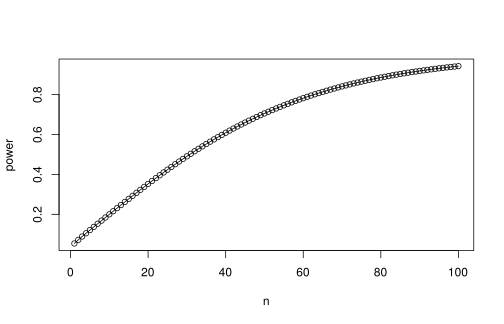
\includegraphics{chapter05_files/figure-latex/unnamed-chunk-15-1.pdf}

\hypertarget{uxbd84uxc0b0uxbd84uxc11d-1}{%
\section{분산분석}\label{uxbd84uxc0b0uxbd84uxc11d-1}}

이제 라틴정방계획법으로 얻은 자료에 대래 분산분석을 적용해 보자.

\begin{Shaded}
\begin{Highlighting}[]
\NormalTok{model}\OtherTok{\textless{}{-}} \FunctionTok{aov}\NormalTok{(y }\SpecialCharTok{\textasciitilde{}}\NormalTok{ trt }\SpecialCharTok{+}\NormalTok{ R }\SpecialCharTok{+}\NormalTok{ C, }\AttributeTok{data=}\NormalTok{df)}
\FunctionTok{summary}\NormalTok{(model)}
\end{Highlighting}
\end{Shaded}

\begin{verbatim}
##             Df Sum Sq Mean Sq F value Pr(>F)   
## trt          4    330    82.5    7.73 0.0025 **
## R            4     68    17.0    1.59 0.2391   
## C            4    150    37.5    3.52 0.0404 * 
## Residuals   12    128    10.7                  
## ---
## Signif. codes:  0 '***' 0.001 '**' 0.01 '*' 0.05 '.' 0.1 ' ' 1
\end{verbatim}

위의 분산분석표에서 추진체(처리)의 효과를 검정하는 F-통계량의 값은 7.7344 이고 p-값은 0.0025이다. 따라서 5\% 유의수준으로 귀무가설을 기각하며 추진체에 따라서 성능이 유의하게 다르다.

\hypertarget{uxb77cuxd2f4uxc815uxbc29uxc758-uxad6cuxcd95}{%
\section{라틴정방의 구축}\label{uxb77cuxd2f4uxc815uxbc29uxc758-uxad6cuxcd95}}

교과서 5.3절에서는 라틴정방 계획으로 실험을 하는 경우 처리를 랜덤하게 배정하는 방법을 설명하고 있다.

패키지 \texttt{agricolae} 에 포함된 함수 \texttt{design.lsd()}를 이용하면 다음과 같이 처리를 랜덤하게 배정해준다.

\begin{Shaded}
\begin{Highlighting}[]
\NormalTok{mytrt }\OtherTok{\textless{}{-}} \FunctionTok{factor}\NormalTok{(}\FunctionTok{c}\NormalTok{(}\StringTok{"A"}\NormalTok{, }\StringTok{"B"}\NormalTok{, }\StringTok{"C"}\NormalTok{, }\StringTok{"D"}\NormalTok{, }\StringTok{"E"}\NormalTok{))}
\NormalTok{mytrt}
\end{Highlighting}
\end{Shaded}

\begin{verbatim}
## [1] A B C D E
## Levels: A B C D E
\end{verbatim}

\begin{Shaded}
\begin{Highlighting}[]
\FunctionTok{design.lsd}\NormalTok{(mytrt)}\SpecialCharTok{$}\NormalTok{sketch}
\end{Highlighting}
\end{Shaded}

\begin{verbatim}
##      [,1] [,2] [,3] [,4] [,5]
## [1,] "C"  "D"  "B"  "A"  "E" 
## [2,] "E"  "A"  "D"  "C"  "B" 
## [3,] "D"  "E"  "C"  "B"  "A" 
## [4,] "B"  "C"  "A"  "E"  "D" 
## [5,] "A"  "B"  "E"  "D"  "C"
\end{verbatim}

함수 \texttt{design.lsd()}는 실행할 때마다 랜덤하게 배정하기 때문에 기록을 위해서 랜덤 seed 를 지정하면
나중에도 동일한 계획을 얻을 수 있다.

\begin{Shaded}
\begin{Highlighting}[]
\FunctionTok{design.lsd}\NormalTok{(mytrt, }\AttributeTok{seed =} \DecValTok{1234}\NormalTok{ )}\SpecialCharTok{$}\NormalTok{sketch}
\end{Highlighting}
\end{Shaded}

\begin{verbatim}
##      [,1] [,2] [,3] [,4] [,5]
## [1,] "C"  "B"  "E"  "A"  "D" 
## [2,] "A"  "E"  "C"  "D"  "B" 
## [3,] "B"  "A"  "D"  "E"  "C" 
## [4,] "D"  "C"  "A"  "B"  "E" 
## [5,] "E"  "D"  "B"  "C"  "A"
\end{verbatim}

\hypertarget{ex53}{%
\chapter{처리 조합의 블럭}\label{ex53}}

\hypertarget{uxc2e4uxd5d8-uxacc4uxd68d-uxad50uxc7ac-uxbd84uxd560uxbc95-i---uxc608uxc81c-5.3---uxd654uxd559uxc57duxd488uxc758-uxc0dduxc131uxb960}{%
\section{실험 계획: 교재 분할법 I - 예제 5.3 - 화학약품의 생성률}\label{uxc2e4uxd5d8-uxacc4uxd68d-uxad50uxc7ac-uxbd84uxd560uxbc95-i---uxc608uxc81c-5.3---uxd654uxd559uxc57duxd488uxc758-uxc0dduxc131uxb960}}

이 실험에서는 화학약품의 생성률에 영향을 미치는 두 요인을 고려한 실험이다.

\begin{itemize}
\tightlist
\item
  반응온도(\texttt{temp}, \(\alpha\)) 3개의 수준
\item
  중간원료 제조회사 (\texttt{company}, \(\beta\)) 3개의 수준
\end{itemize}

이 실험에서는 9개의 처리를 먼저 랜덤하게 선택하고 선택된 처리 하에서 실험을 2번 반복하였다.
따라서 처리의 조합이 블럭효과(\texttt{block}, \(\rho\))로 나타난다.

\[ x_{ijk} = \mu + \alpha_i + \beta_j + \rho_{ij} + e_{2(ijk)} \]

위의 모형식에서 상호작용 효과 \((\alpha \beta)_{ij}\) 와 1차 랜덤화에 의한 오차 \(e_{1(ij)}\) 는 교락되어
블럭효과 \(\rho_{ij}\)에 합쳐저서 나타난다.

\[ \rho_{ij} = e_{1(ij)} + (\alpha \beta)_{ij}  \]

이러한 경우 블럭효과 \(\rho_{ij}\)는 임의효과가 된다.

\begin{equation}
\rho_{ij}   \sim N(0, \sigma_1^2), \quad e_{2(ijk)} \sim N(0, \sigma_2^2) 
\label{eq:cond1}
\end{equation}

\hypertarget{uxc790uxb8ccuxc758-uxad6cuxc131-2}{%
\section{자료의 구성}\label{uxc790uxb8ccuxc758-uxad6cuxc131-2}}

이제 실험자료를 입력하여 데이터프레임으로 만들어 보자

\begin{Shaded}
\begin{Highlighting}[]
\NormalTok{temp}\OtherTok{\textless{}{-}} \FunctionTok{as.factor}\NormalTok{(}\FunctionTok{rep}\NormalTok{(}\FunctionTok{c}\NormalTok{(}\StringTok{"A1"}\NormalTok{,}\StringTok{"A2"}\NormalTok{, }\StringTok{"A3"}\NormalTok{), }\AttributeTok{each=}\DecValTok{2}\NormalTok{, }\AttributeTok{times=}\DecValTok{3}\NormalTok{))}
\NormalTok{company}\OtherTok{\textless{}{-}} \FunctionTok{as.factor}\NormalTok{(}\FunctionTok{rep}\NormalTok{(}\FunctionTok{c}\NormalTok{(}\StringTok{"B1"}\NormalTok{, }\StringTok{"B2"}\NormalTok{, }\StringTok{"B3"}\NormalTok{), }\AttributeTok{each=}\DecValTok{6}\NormalTok{))}

\NormalTok{y }\OtherTok{\textless{}{-}}\FunctionTok{c}\NormalTok{( }\FloatTok{81.0}\NormalTok{, }\FloatTok{80.2}\NormalTok{, }\FloatTok{84.1}\NormalTok{, }\FloatTok{83.2}\NormalTok{, }\FloatTok{85.2}\NormalTok{, }\FloatTok{86.1}\NormalTok{,}
       \FloatTok{83.3}\NormalTok{, }\FloatTok{82.7}\NormalTok{, }\FloatTok{86.2}\NormalTok{, }\FloatTok{85.4}\NormalTok{, }\FloatTok{86.6}\NormalTok{, }\FloatTok{87.2}\NormalTok{,}
       \FloatTok{81.3}\NormalTok{, }\FloatTok{81.9}\NormalTok{, }\FloatTok{83.2}\NormalTok{, }\FloatTok{84.2}\NormalTok{, }\FloatTok{86.0}\NormalTok{, }\FloatTok{86.4}\NormalTok{) }

\NormalTok{df}\OtherTok{\textless{}{-}} \FunctionTok{data.frame}\NormalTok{(temp, company, y)}
\NormalTok{df}
\end{Highlighting}
\end{Shaded}

\begin{verbatim}
##    temp company    y
## 1    A1      B1 81.0
## 2    A1      B1 80.2
## 3    A2      B1 84.1
## 4    A2      B1 83.2
## 5    A3      B1 85.2
## 6    A3      B1 86.1
## 7    A1      B2 83.3
## 8    A1      B2 82.7
## 9    A2      B2 86.2
## 10   A2      B2 85.4
## 11   A3      B2 86.6
## 12   A3      B2 87.2
## 13   A1      B3 81.3
## 14   A1      B3 81.9
## 15   A2      B3 83.2
## 16   A2      B3 84.2
## 17   A3      B3 86.0
## 18   A3      B3 86.4
\end{verbatim}

\hypertarget{uxc2dcuxac01uxc801-uxbd84uxc11d-2}{%
\section{시각적 분석}\label{uxc2dcuxac01uxc801-uxbd84uxc11d-2}}

일단 각 처리에 대한 관측값의 평균을 구해보자.

\begin{Shaded}
\begin{Highlighting}[]
\NormalTok{dfsum }\OtherTok{\textless{}{-}}\NormalTok{ df }\SpecialCharTok{\%\textgreater{}\%} \FunctionTok{group\_by}\NormalTok{(temp, company)  }\SpecialCharTok{\%\textgreater{}\%}  \FunctionTok{summarise}\NormalTok{(}\AttributeTok{mean=}\FunctionTok{mean}\NormalTok{(y),  }\AttributeTok{sd=}\FunctionTok{sd}\NormalTok{(y))}
\end{Highlighting}
\end{Shaded}

\begin{verbatim}
## `summarise()` has grouped output by 'temp'. You can override using the `.groups` argument.
\end{verbatim}

\begin{Shaded}
\begin{Highlighting}[]
\NormalTok{dfsum}
\end{Highlighting}
\end{Shaded}

\begin{verbatim}
## # A tibble: 9 x 4
## # Groups:   temp [3]
##   temp  company  mean    sd
##   <fct> <fct>   <dbl> <dbl>
## 1 A1    B1       80.6 0.566
## 2 A1    B2       83   0.424
## 3 A1    B3       81.6 0.424
## 4 A2    B1       83.6 0.636
## 5 A2    B2       85.8 0.566
## 6 A2    B3       83.7 0.707
## 7 A3    B1       85.6 0.636
## 8 A3    B2       86.9 0.424
## 9 A3    B3       86.2 0.283
\end{verbatim}

이제 처리의 평균값을 가지고 온도에 따른 변화를 살펴보자. 이 경우 제조회사 원료에 대해서는 색깔을 다르게 하여 상호작용 효과도 볼 수 있다.

아래 상호작용 그림을 보면 온도에 따라서 화학약품의 생성률이 크게 변하는 것을 알 수 있다. 유의한 상호작용은 관측되지 않는다.

\begin{Shaded}
\begin{Highlighting}[]
\NormalTok{dfsum }\SpecialCharTok{\%\textgreater{}\%} 
  \FunctionTok{ggplot}\NormalTok{(}\FunctionTok{aes}\NormalTok{(}\AttributeTok{x =}\NormalTok{ temp  , }\AttributeTok{y =}\NormalTok{ mean,  }\AttributeTok{color=}\NormalTok{company)) }\SpecialCharTok{+}
   \FunctionTok{geom\_line}\NormalTok{(}\FunctionTok{aes}\NormalTok{(}\AttributeTok{group =}\NormalTok{ company)) }\SpecialCharTok{+}   \FunctionTok{geom\_point}\NormalTok{()}
\end{Highlighting}
\end{Shaded}

\includegraphics{chapter05_files/figure-latex/unnamed-chunk-24-1.pdf}

함수 \texttt{interaction.plot()은}상호작용 그림을 평균값을 계산하지 않고 원래 자료를 이용하여 다음과 같이 그릴 수 있다.

\begin{Shaded}
\begin{Highlighting}[]
\FunctionTok{with}\NormalTok{(df, }\FunctionTok{interaction.plot}\NormalTok{(}\AttributeTok{x.factor =}\NormalTok{ temp, }\AttributeTok{trace.factor =}\NormalTok{ company,  }\AttributeTok{response =}\NormalTok{ y))}
\end{Highlighting}
\end{Shaded}

\includegraphics{chapter05_files/figure-latex/unnamed-chunk-25-1.pdf}

\begin{rmdnote}
위에서 함수 \texttt{with()} 은 이용하고자 하는 변수가 있는 데이터프레임을 지정하는데사용한다.
함수 \texttt{with()}의 첫 번쨰 인자는 앞의 예제와 같이 \texttt{df} 와 같은 데이터 프레임을 지정한다.
두 번째 인자에는 함수를 이용한 명령문을 넣어준다. 앞의 프로그램에서 함수 \texttt{interaction.plot()}
안에서 사용된 변수들( \texttt{temp},\texttt{company},\texttt{y})들은 데이터프레임 \texttt{df}에 있는 변수들이다.
\end{rmdnote}

이제 제조회사에 따른 변화를 살펴보자. 제조회사에 따른 생성률의 변화는 크지 않다.

\begin{Shaded}
\begin{Highlighting}[]
\FunctionTok{with}\NormalTok{(df, }\FunctionTok{interaction.plot}\NormalTok{(}\AttributeTok{x.factor =}\NormalTok{ company, }\AttributeTok{trace.factor =}\NormalTok{temp ,  }\AttributeTok{response =}\NormalTok{ y))}
\end{Highlighting}
\end{Shaded}

\includegraphics{chapter05_files/figure-latex/unnamed-chunk-27-1.pdf}

\hypertarget{uxbd84uxc0b0uxbd84uxc11d-2}{%
\section{분산분석}\label{uxbd84uxc0b0uxbd84uxc11d-2}}

이제 분산분석을 하여 처리의 효과에 대한 검정을 해보자. 실험에서 각 처리의 조합을
블럭으로 해주어야 한다.

다음 \texttt{anova} 함수에서 두 처리의 조합을 \texttt{temp:company} 로 표시한다. 사실 \texttt{temp:company}는 두 처리
\texttt{temp}와 \texttt{company}의 상호작용(interaction)을 의미한다. 다음으로 처리의 조합 \texttt{temp:company} 이
임의효과라는 것을 \texttt{Error(temp:company)}와 같이 지정해 준다.

\begin{Shaded}
\begin{Highlighting}[]
\NormalTok{model}\OtherTok{\textless{}{-}} \FunctionTok{aov}\NormalTok{(y }\SpecialCharTok{\textasciitilde{}}\NormalTok{ temp }\SpecialCharTok{+}\NormalTok{ company }\SpecialCharTok{+} \FunctionTok{Error}\NormalTok{(temp}\SpecialCharTok{:}\NormalTok{company), }\AttributeTok{data=}\NormalTok{df)}
\end{Highlighting}
\end{Shaded}

\begin{verbatim}
## Warning in aov(y ~ temp + company + Error(temp:company), data = df): Error()
## model is singular
\end{verbatim}

\begin{Shaded}
\begin{Highlighting}[]
\FunctionTok{summary}\NormalTok{(model)}
\end{Highlighting}
\end{Shaded}

\begin{verbatim}
## 
## Error: temp:company
##           Df Sum Sq Mean Sq F value  Pr(>F)    
## temp       2   61.8   30.91    85.7 0.00052 ***
## company    2   12.0    5.98    16.6 0.01157 *  
## Residuals  4    1.4    0.36                    
## ---
## Signif. codes:  0 '***' 0.001 '**' 0.01 '*' 0.05 '.' 0.1 ' ' 1
## 
## Error: Within
##           Df Sum Sq Mean Sq F value Pr(>F)
## Residuals  9   2.57   0.286
\end{verbatim}

위의 분산분석표에서 온도의 효과를 검정하는 F-통계량의 값은 85.7211 이고 p-값은 \ensuremath{5.1982\times 10^{-4}}이다. 따라서 5\% 유의수준으로 귀무가설을 기각하며 온도에 따라서 생성률이 매우 유의하게 다르다.

온도의 효과를 검정하는 F-통계량의 값은 16.5917 이고 p-값은 0.0116이다. 따라서 5\% 유의수준으로 귀무가설을 기각하며 원료 제조회사에 따라서도 생성률이 유의하게 다르다.

\hypertarget{uxbe14uxb7eduxc744-uxace0uxb824uxd558uxc9c0-uxc54auxb294-uxacbduxc6b0}{%
\section{블럭을 고려하지 않는 경우}\label{uxbe14uxb7eduxc744-uxace0uxb824uxd558uxc9c0-uxc54auxb294-uxacbduxc6b0}}

만약에 처리 조합으로 생긴 블럭효과를 고려하지 않으면 어떤 일이 일어날까?

만약 생성률 실험자료를 \textbf{완전 랜덤화 이원배치법}에 의하여 얻은 자료라고 생각한다면 반복이 있으므로
상호작용 효과를 추론할 수 있다. 따라서 상호작용 효과를 고정효과로 놓고 분산분석을 적용할 것이다.

\begin{equation}
\rho_{ij}  = (\alpha \beta)_{ij} : \text{ fixed effect }, \quad e_{2(ijk)} \sim N(0, \sigma_2^2) 
\label{eq:cond2}
\end{equation}

아래 프로그램은 상호작용 효과를 고정효과로 생각한 것이다.

\begin{Shaded}
\begin{Highlighting}[]
\NormalTok{model2}\OtherTok{\textless{}{-}} \FunctionTok{aov}\NormalTok{(y }\SpecialCharTok{\textasciitilde{}}\NormalTok{ temp }\SpecialCharTok{+}\NormalTok{ company }\SpecialCharTok{+}\NormalTok{ temp}\SpecialCharTok{:}\NormalTok{company, }\AttributeTok{data=}\NormalTok{df)}
\FunctionTok{summary}\NormalTok{(model2)}
\end{Highlighting}
\end{Shaded}

\begin{verbatim}
##              Df Sum Sq Mean Sq F value  Pr(>F)    
## temp          2   61.8   30.91  108.24 5.1e-07 ***
## company       2   12.0    5.98   20.95 0.00041 ***
## temp:company  4    1.4    0.36    1.26 0.35267    
## Residuals     9    2.6    0.29                    
## ---
## Signif. codes:  0 '***' 0.001 '**' 0.01 '*' 0.05 '.' 0.1 ' ' 1
\end{verbatim}

분산분석의 결과는 위와 같으며 온도와 제조회사에 대한 F-검정 통계량을 보면 임의효과 모형에서 나온
것보다 크다. 이는 F-검정 통계량을 만들 때 분모에 사용된 평균 오차제곱합 \(MS_E\)와 자유도가 달라서 나타나는 현상이다. 또한 자유도도

두 모형에서 온도에 대한 F-검정의 차이를 보자.

\begin{longtable}[]{@{}lllll@{}}
\toprule
모형 & \texttt{anova} 항 & \(MS_A\) & \(MS_E\) & \(F_0\)\tabularnewline
\midrule
\endhead
임의효과 모형 {[}식 \eqref{eq:cond1}{]} & \texttt{Error(temp:company)} & 30.9072 & 0.3606 & 85.7211\tabularnewline
고정효과 모형 {[}식 \eqref{eq:cond2}{]} & \texttt{temp:company} & 30.9072 & 0.2856 & 108.2354\tabularnewline
\bottomrule
\end{longtable}

위의 표에서와 같이 실험계획에 따라서 나누어 주는 평균 오차제곱합 \(MS_E\)와 자유도가 다르기 때문에 검정의 결과가 다르게 나타난다.

\begin{rmdcaution}
실험계획에서 통계적 추론을 하는 경우 자료의 구조는 같아도 실험의 방법(랜덤화의 방법)이 다르면 가설검정의 방법이 다르다.

따라서 실험의 방법에 따른 적절한 통계적 추론 방법을 선택하는 것이 중요하다.
\end{rmdcaution}

\hypertarget{uxd63cuxd569uxbaa8uxd615-1}{%
\section{혼합모형}\label{uxd63cuxd569uxbaa8uxd615-1}}

처리들의 조합을 임의효과로 보는 모형 \eqref{eq:cond1} 을 \texttt{lmer}로 적합시키는 프로그램은 다음과 같다.

분산분석 결과는 \texttt{anova()} 에서 임의효과 \texttt{Error(temp:company)}를 사용하는 결과와 동일하다.

\begin{Shaded}
\begin{Highlighting}[]
\NormalTok{fit }\OtherTok{\textless{}{-}} \FunctionTok{lmer}\NormalTok{(y }\SpecialCharTok{\textasciitilde{}}\NormalTok{ temp }\SpecialCharTok{+}\NormalTok{ company }\SpecialCharTok{+}\NormalTok{ (}\DecValTok{1} \SpecialCharTok{|}\NormalTok{ temp}\SpecialCharTok{:}\NormalTok{company ), }\AttributeTok{data =}\NormalTok{ df)}
\FunctionTok{summary}\NormalTok{(fit)}
\end{Highlighting}
\end{Shaded}

\begin{verbatim}
## Linear mixed model fit by REML. t-tests use Satterthwaite's method [
## lmerModLmerTest]
## Formula: y ~ temp + company + (1 | temp:company)
##    Data: df
## 
## REML criterion at convergence: 29.4
## 
## Scaled residuals: 
##     Min      1Q  Median      3Q     Max 
## -1.5203 -0.4673 -0.0711  0.7760  1.2014 
## 
## Random effects:
##  Groups       Name        Variance Std.Dev.
##  temp:company (Intercept) 0.0375   0.194   
##  Residual                 0.2856   0.534   
## Number of obs: 18, groups:  temp:company, 9
## 
## Fixed effects:
##             Estimate Std. Error     df t value Pr(>|t|)    
## (Intercept)   80.911      0.316  4.000  255.67  1.4e-09 ***
## tempA2         2.650      0.347  4.000    7.64   0.0016 ** 
## tempA3         4.517      0.347  4.000   13.03   0.0002 ***
## companyB2      1.933      0.347  4.000    5.58   0.0051 ** 
## companyB3      0.533      0.347  4.000    1.54   0.1988    
## ---
## Signif. codes:  0 '***' 0.001 '**' 0.01 '*' 0.05 '.' 0.1 ' ' 1
## 
## Correlation of Fixed Effects:
##           (Intr) tempA2 tempA3 cmpnB2
## tempA2    -0.548                     
## tempA3    -0.548  0.500              
## companyB2 -0.548  0.000  0.000       
## companyB3 -0.548  0.000  0.000  0.500
\end{verbatim}

\begin{Shaded}
\begin{Highlighting}[]
\FunctionTok{anova}\NormalTok{(fit)}
\end{Highlighting}
\end{Shaded}

\begin{verbatim}
## Type III Analysis of Variance Table with Satterthwaite's method
##         Sum Sq Mean Sq NumDF DenDF F value  Pr(>F)    
## temp      49.0   24.48     2     4    85.7 0.00052 ***
## company    9.5    4.74     2     4    16.6 0.01157 *  
## ---
## Signif. codes:  0 '***' 0.001 '**' 0.01 '*' 0.05 '.' 0.1 ' ' 1
\end{verbatim}

\hypertarget{ex54}{%
\chapter{Split-Plot desgin}\label{ex54}}

\hypertarget{uxc2e4uxd5d8-uxacc4uxd68d-uxad50uxc7ac-uxbd84uxd560uxbc95-ii---uxc608uxc81c-5.4---uxc804uxc790uxc81cuxd488-uxc218uxba85}{%
\section{실험 계획: 교재 분할법 II - 예제 5.4 - 전자제품 수명}\label{uxc2e4uxd5d8-uxacc4uxd68d-uxad50uxc7ac-uxbd84uxd560uxbc95-ii---uxc608uxc81c-5.4---uxc804uxc790uxc81cuxd488-uxc218uxba85}}

전자부품의 수명이 온도(580, 600, 620, 640도)와 시간(5, 10, 15분)에 의해 어떤 영향을 받는지에 대한 실험이다.

이 실험은 split-plot 설계를 적용하여 관측값을 얻었다. 온도를 먼저 랜덤하게 선택하고 선택된 온도에서 3개의 가열 시간에 대한 실험을 임의 순서로 진행하였다. 또한 각 실험은 3번 반복 하였다.

\begin{itemize}
\tightlist
\item
  온도 (\texttt{temp}, \(\alpha\)) : 주구, main plot - 1차 랜덤화 요인
\item
  시간 (\texttt{time}, \(\beta\)) : 분할구, split-plot, sub-plot - 2차 랜덤화 요인
\item
  반복 (\texttt{rep}, \(r\)) : 반복 요인
\end{itemize}

\begin{equation}
x_{ijk} = \mu + r_k + \alpha_i + \gamma_{ik} + \beta_j + (\alpha \beta)_{ij} + e_{2(ijk)} 
\label{eq:splitplot}
\end{equation}

위의 모형식에서 반복과 온도의 상호작용 효과 \(( \alpha r)_{ik}\) 와 1차 랜덤화에 의한 오차 \(e_{1(ik)}\) 는 교락되어
블럭효과 \(\gamma_{ik}\)에 합쳐저서 나타난다.

\[ \gamma_{ik}  =  (\alpha r)_{ik} + e_{1(ik)}  \]

\hypertarget{uxc790uxb8ccuxc758-uxad6cuxc131-3}{%
\section{자료의 구성}\label{uxc790uxb8ccuxc758-uxad6cuxc131-3}}

이제 실험자료를 입력하여 데이터프레임으로 만들어 보자

\begin{Shaded}
\begin{Highlighting}[]
\NormalTok{rep}\OtherTok{\textless{}{-}} \FunctionTok{as.factor}\NormalTok{(}\FunctionTok{rep}\NormalTok{(}\FunctionTok{c}\NormalTok{(}\DecValTok{1}\SpecialCharTok{:}\DecValTok{3}\NormalTok{), }\AttributeTok{each=}\DecValTok{12}\NormalTok{))}
\NormalTok{temp}\OtherTok{\textless{}{-}} \FunctionTok{as.factor}\NormalTok{(}\FunctionTok{rep}\NormalTok{(}\FunctionTok{c}\NormalTok{(}\DecValTok{580}\NormalTok{, }\DecValTok{600}\NormalTok{, }\DecValTok{620}\NormalTok{, }\DecValTok{640}\NormalTok{), }\AttributeTok{each=}\DecValTok{3}\NormalTok{, }\AttributeTok{times=}\DecValTok{3}\NormalTok{))}
\NormalTok{time}\OtherTok{\textless{}{-}} \FunctionTok{as.factor}\NormalTok{(}\FunctionTok{rep}\NormalTok{(}\FunctionTok{c}\NormalTok{(}\DecValTok{5}\NormalTok{, }\DecValTok{10}\NormalTok{, }\DecValTok{15}\NormalTok{), }\AttributeTok{times=}\DecValTok{12}\NormalTok{))}

\NormalTok{y }\OtherTok{\textless{}{-}}\FunctionTok{c}\NormalTok{(}\DecValTok{217}\NormalTok{, }\DecValTok{233}\NormalTok{, }\DecValTok{175}\NormalTok{, }\DecValTok{158}\NormalTok{, }\DecValTok{138}\NormalTok{, }\DecValTok{152}\NormalTok{, }\DecValTok{229}\NormalTok{, }\DecValTok{186}\NormalTok{, }\DecValTok{155}\NormalTok{, }\DecValTok{223}\NormalTok{, }\DecValTok{227}\NormalTok{, }\DecValTok{156}\NormalTok{,}
        \DecValTok{188}\NormalTok{, }\DecValTok{201}\NormalTok{, }\DecValTok{195}\NormalTok{, }\DecValTok{126}\NormalTok{, }\DecValTok{130}\NormalTok{, }\DecValTok{147}\NormalTok{, }\DecValTok{160}\NormalTok{, }\DecValTok{170}\NormalTok{, }\DecValTok{161}\NormalTok{, }\DecValTok{201}\NormalTok{, }\DecValTok{181}\NormalTok{, }\DecValTok{172}\NormalTok{,}
        \DecValTok{162}\NormalTok{, }\DecValTok{170}\NormalTok{, }\DecValTok{213}\NormalTok{, }\DecValTok{122}\NormalTok{, }\DecValTok{185}\NormalTok{, }\DecValTok{180}\NormalTok{, }\DecValTok{167}\NormalTok{, }\DecValTok{181}\NormalTok{, }\DecValTok{182}\NormalTok{, }\DecValTok{182}\NormalTok{, }\DecValTok{201}\NormalTok{, }\DecValTok{199}\NormalTok{) }

\NormalTok{df }\OtherTok{\textless{}{-}} \FunctionTok{data.frame}\NormalTok{(rep, temp, time, y)}
\end{Highlighting}
\end{Shaded}

함수 \texttt{xtab} 을 이용하면 반복에 따라서 자료 구조를 쉽게 볼 수 있다.

\begin{Shaded}
\begin{Highlighting}[]
\FunctionTok{xtabs}\NormalTok{( y }\SpecialCharTok{\textasciitilde{}}\NormalTok{time }\SpecialCharTok{+}\NormalTok{ temp }\SpecialCharTok{+}\NormalTok{ rep, df)}
\end{Highlighting}
\end{Shaded}

\begin{verbatim}
## , , rep = 1
## 
##     temp
## time 580 600 620 640
##   5  217 158 229 223
##   10 233 138 186 227
##   15 175 152 155 156
## 
## , , rep = 2
## 
##     temp
## time 580 600 620 640
##   5  188 126 160 201
##   10 201 130 170 181
##   15 195 147 161 172
## 
## , , rep = 3
## 
##     temp
## time 580 600 620 640
##   5  162 122 167 182
##   10 170 185 181 201
##   15 213 180 182 199
\end{verbatim}

\hypertarget{uxc2dcuxac01uxc801-uxbd84uxc11d-3}{%
\section{시각적 분석}\label{uxc2dcuxac01uxc801-uxbd84uxc11d-3}}

이제 온도의 수준에 따른 변화를 볼 수 있는 그림을 그려보자. 온도가 증가하면서 수명이 줄어들었다가 다시 늘어나는 현상을 볼 수 있다.

\begin{Shaded}
\begin{Highlighting}[]
\FunctionTok{with}\NormalTok{(df, }\FunctionTok{interaction.plot}\NormalTok{(}\AttributeTok{x.factor =}\NormalTok{ temp, }\AttributeTok{trace.factor =}\NormalTok{ time, }\AttributeTok{response =}\NormalTok{ y))}
\end{Highlighting}
\end{Shaded}

\includegraphics{chapter05_files/figure-latex/unnamed-chunk-37-1.pdf}

가열시간의 수준에 따른 변화를 볼 수 있는 그림을 그려보자. 가열시간이 증가하더러도 수명이 크게 변하지 않는 것을 알 수 있다.

\begin{Shaded}
\begin{Highlighting}[]
\FunctionTok{with}\NormalTok{(df, }\FunctionTok{interaction.plot}\NormalTok{(}\AttributeTok{x.factor =}\NormalTok{ time, }\AttributeTok{trace.factor =}\NormalTok{ temp, }\AttributeTok{response =}\NormalTok{ y))}
\end{Highlighting}
\end{Shaded}

\includegraphics{chapter05_files/figure-latex/unnamed-chunk-38-1.pdf}

\hypertarget{uxbd84uxc0b0uxbd84uxc11d-3}{%
\section{분산분석}\label{uxbd84uxc0b0uxbd84uxc11d-3}}

이제 모형식 \eqref{eq:splitplot} 에 대한 분산분석을 실시해 보자.

여기서 유의할 점은 모형식 \eqref{eq:splitplot} 에서 블럭효과 \(\gamma_{ik}\)는 임의효과로 생각하며 반복 수준과 온도 수준의 조합이다. 따라서 블럭효과 \(\gamma_{ik}\) 에 대한 항을 \texttt{Error(rep:temp)}로 사용한다.

\[ \gamma_{ik} \sim N(0,\sigma^2_1), \quad e_{2(ijk)} \sim N(0, \sigma^2_E) \]

\begin{Shaded}
\begin{Highlighting}[]
\NormalTok{model}\OtherTok{\textless{}{-}} \FunctionTok{aov}\NormalTok{(y }\SpecialCharTok{\textasciitilde{}}\NormalTok{ rep }\SpecialCharTok{+}\NormalTok{ temp}\SpecialCharTok{*}\NormalTok{time }\SpecialCharTok{+} \FunctionTok{Error}\NormalTok{(rep}\SpecialCharTok{:}\NormalTok{temp), }\AttributeTok{data=}\NormalTok{df)}
\end{Highlighting}
\end{Shaded}

\begin{verbatim}
## Warning in aov(y ~ rep + temp * time + Error(rep:temp), data = df): Error()
## model is singular
\end{verbatim}

\begin{Shaded}
\begin{Highlighting}[]
\FunctionTok{summary}\NormalTok{(model)}
\end{Highlighting}
\end{Shaded}

\begin{verbatim}
## 
## Error: rep:temp
##           Df Sum Sq Mean Sq F value Pr(>F)   
## rep        2   1963     981    3.32  0.107   
## temp       3  12494    4165   14.09  0.004 **
## Residuals  6   1774     296                  
## ---
## Signif. codes:  0 '***' 0.001 '**' 0.01 '*' 0.05 '.' 0.1 ' ' 1
## 
## Error: Within
##           Df Sum Sq Mean Sq F value Pr(>F)
## time       2    566     283    0.46   0.64
## temp:time  6   2600     433    0.70   0.66
## Residuals 16   9933     621
\end{verbatim}

분산분석표에서 온도의 효과를 검정하는 F-통계량의 값은 14.0865 이고 p-값은 0.004이다. 따라서 5\% 유의수준으로 귀무가설을 기각하며 온도에 따라서 제품의 수명이 유의하게 다르다.

가열시간의 효과를 검정하는 F-통계량의 값은 0.456 이고 p-값은 0.6418이다. 따라서 5\% 유의수준으로 귀무가설을 기각할 수 없으며 가열시간에 따라서 제품의 수명이 다르지 않다.

온도와 가열시간의 상호작용 효과를 검정하는 F-통계량의 값은 0.6981 이고 p-값은 0.6551이다. 따라서 5\% 유의수준으로 귀무가설을 기각할 수 없으며 상호작용은 유의하지 않다.

  \bibliography{book.bib,packages.bib}

\end{document}
